\documentclass[10pt,fleqn]{beamer}

\usepackage[english]{babel}
\usepackage[T1]{fontenc}
\usepackage[utf8]{inputenc}

\usepackage{multirow} % To merge cels horizontaly

\usepackage{algpseudocode}
\usepackage{multicol} % para utilizar ambiente "multicols"
\usepackage{pdfpages} % para incluir paginas de documentos PDFs
\usepackage{color, amsmath}
\usepackage{subfigure}
\usepackage{graphicx} % para incluir figuras
\usepackage[ruled,longend]{algorithm2e} % para escrever algoritmos
\usepackage{ulem}       % para trocar a fonte?

\definecolor{defblue}{rgb}{0.2, 0.2, 0.7}
\definecolor{defred}{rgb}{0.4, 0.0, 0.0}
\definecolor{defgreen}{rgb}{0.0, 0.4, 0.0}

\definecolor{ninfagreen}{rgb}{0.168, 0.541, 0.569} % changed this

\newcommand{\spc}{\phantom{a}}

% algpseudocode
\newsavebox{\ieeealgbox}
\newenvironment{boxedalgorithmic}
  {\begin{lrbox}{\ieeealgbox}
   \begin{minipage}{\dimexpr\columnwidth-2\fboxsep-2\fboxrule}
   \begin{algorithmic}}
  {\end{algorithmic}
   \end{minipage}
   \end{lrbox}\noindent\fbox{\usebox{\ieeealgbox}}}

% Set left ident of equations
\setlength{\mathindent}{4pt}

\newcommand{\mydef}[1]{{\vspace{8pt} \large \color{defblue} #1}}
\newcommand{\myred}[1]{{\bf \color{defred} #1}}
\newcommand{\mygreen}[1]{{\bf \color{defgreen} #1}}

\renewcommand{\rmdefault}{put} % Utopia Font
\renewcommand{\sfdefault}{put} % Utopia Font
\renewcommand{\emph}[1]{ {\bf #1} }

% Scale Equations
\newcommand*{\Scale}[2][4]{\scalebox{#1}{$#2$}}%

\newcommand{\litem}[1]{
  \item{#1 \vspace{9pt}}
}

%\usetheme{Berkeley}
%\usetheme{Hannover}
%\usetheme{Marcos}
%\usetheme{default}
\usetheme{Boadilla}
%\usetheme{Pittsburgh}

%\useinnertheme{rectangles}
%\useoutertheme{tree}
%\setbeamercolor{separation line}{use=structure,bg=structure.fg!50!bg}

%\usecolortheme{dolphin}
%\usecolortheme{seahorse}

\beamertemplatenavigationsymbolsempty

% Escrita dos algoritmos
\SetKwInput{KwIn}{Entrada}
\SetKwInput{KwOut}{Saída}
\SetKwFor{While}{enquanto}{faça:}{fim}
\SetKwFor{For}{para}{faça:}{fim}
\SetKwBlock{Begin}{início}{fim}
\SetKwIF{If}{ElseIf}{Else}{se}{então}{senão se}{senão}{fim}

\newcommand{\bigbullet}{\,\begin{picture}(-1,1)(-1,-2)\circle*{5}\end{picture}\ }
\newcommand{\termo}[1]{\textbf{#1}}
\newcommand{\titulo}[1]{\centering \LARGE \vfill \textcolor{defblue}{\textbf{#1}} \vfill }

\newcommand{\chamada}[1]{
  \textcolor{ninfagreen}{\textbf{#1}}
  \vspace{10pt}
}

%\title{Um Estudo da Eficiência da Autocentralidade no Problema de Isomorfismo de Grafos}
\title[]{A shuffled complex evolution algorithm for
the multidimensional knapsack problem using core concept}
\subtitle{}
\author{Marcos Daniel Baroni}
\institute[NINFA]{}
\date[Vitória, 24/08/2015]{Vitória, 24 de agosto de 2015}
\subject{}

% Figura de fundo
\setbeamercolor{background canvas}{bg=white}
\setbeamertemplate{background}{
\includegraphics[width=\paperwidth,bb=0 0 1036 777]{fundo.png}}

% Posição dos títulos dos slides
\addtobeamertemplate{frametitle}{\vskip 2.5ex }{}
\addtobeamertemplate{frametitle}{\bf }{}

\begin{document}

\definecolor{beamer@blendedblue}{rgb}{0.168, 0.541, 0.569} % changed this

%\setbeamercolor{normal text}{fg=black,bg=white}
%\setbeamercolor{alerted text}{fg=red}
%\setbeamercolor{example text}{fg=green!50!black}

%\setbeamercolor{structure}{fg=beamer@blendedblue}

%\setbeamercolor{background canvas}{parent=normal text}
%\setbeamercolor{background}{parent=background canvas}

%\setbeamercolor{palette primary}{fg=yellow,bg=yellow} % changed this
%\setbeamercolor{palette secondary}{use=structure,fg=structure.fg!100!green} % changed this
%\setbeamercolor{palette tertiary}{use=structure,fg=structure.fg!100!green} % changed this

\begin{frame}
  \titlepage
\end{frame}

\begin{frame}
  \frametitle{Sumário}
  \begin{itemize}
    \litem{Introduction}
	\litem{The core concept for MKP}
	\litem{The shuffled complex evolution (SCE)}
	\litem{SCE for the MKP}
	\litem{Computational experiments}
	\litem{Conclusions and future remarks}
  \end{itemize}
\end{frame}

\section{The core concept for MKP}

\begin{frame}
	\frametitle{The core concept for MKP}
	\framesubtitle{The multidimensional knapsack problem}
The multidimensional knapsack problem (MKP) is a strongly NP-hard combinatorial
optimization problem which can be viewed as a resource allocation problem and
defined as follows:
  \begin{columns}[T]
    % Primeira coluna
	  \begin{column}{.5\textwidth}
      \begin{block}{Modelagem matemática}
	    { \footnotesize
\begin{align*}
  \text{maximize} & \sum_{j=1}^n p_j x_j \\
  \text{subject to} & \sum_{j=1}^n w_{ij} x_j \leqslant c_i \quad i \in \{1, \ldots, m\}\\
   & x_j \in \{0, 1\}, \quad j \in \{1, \ldots, n\}.
\end{align*}
		}
      \end{block}
    \end{column} \pause
    % Segunda coluna
    \begin{column}{.5\textwidth}
	  \begin{center}
        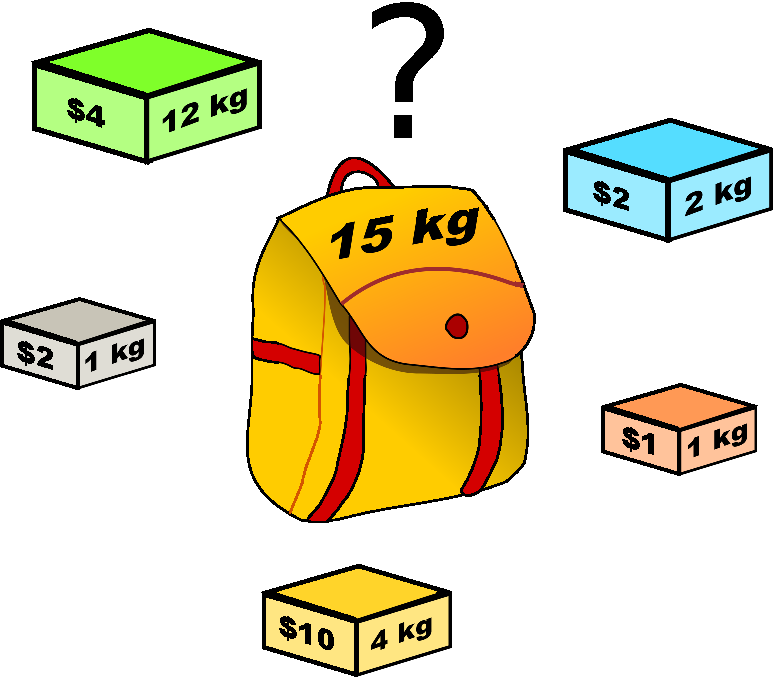
\includegraphics[scale=0.3]{knapsack}
	  \end{center}
    \end{column}
  \end{columns}
\end{frame}

\begin{frame}
	\frametitle{The core concept for MKP}
  \framesubtitle{}
  The {\bf core} is a set of items which are hard to decide if they
are or not selected in good solutions.
  % Definição geral de um problema de otimização:
\begin{align*}
		\text{\bf efficiency:} \qquad e_i = \frac{p_i}{w_i}
\end{align*} \pause
	high efficiency $\rightarrow x_i = 1$ \\
	low efficiency \phantom{.} $\rightarrow x_i = 0$ \\
	mid efficiency $\rightarrow x_i = ?$\\
	  \begin{center}
        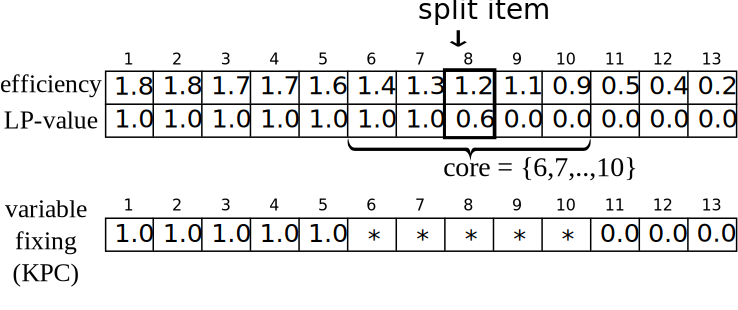
\includegraphics[scale=0.5]{../imgs/kp_3}
	  \end{center}
\end{frame}

\begin{frame}
	\frametitle{The core concept for MKP}
The core for KP extended to MKP:
  % Definição geral de um problema de otimização:
\begin{displaymath}
	\qquad e_j(simple) = \frac{p_j}{\sum_{i=1}^{m} w_{ij}}
\end{displaymath}
{\bf Problem:} orders of magnitude of the constraints are not
considered. \\
\pause
{\bf Solution:} Introduce a relevance factor for each constraint:
\begin{displaymath}
	\qquad e_j(relevance) = \frac{p_j}{\sum_{i=1}^{m} r_i . w_{ij}}
\end{displaymath}
Values of an optimal solution to the dual problem
(relates to the importance of each resource).
\end{frame}

\begin{frame}
	\frametitle{The core concept for MKP}
The KP Core problem (KPC) is defined as
      \begin{block}{Modelagem matemática}
	    { \footnotesize
\begin{align*}
  \text{maximize} & \sum_{j \in C} p_j x_j  + \tilde{p}\\
  \text{subject to} & \sum_{j \in C} w_{j} x_j \leqslant c - \tilde{w}\\
  & x_j \in \{0, 1\}, \quad j \in C.
\end{align*}
		}
      \end{block}
\end{frame}


\begin{frame}
	\frametitle{The shuffled complex evolution (SCE)}
The shuffled complex evolution is a population
based evolutionary optimization algorithm that regards a natural 
evolution happening simultaneously in independent communities: \\ \pause
\vfill
The whole population is partitioned in $N$ {\bf complexes}.
Each complex has $M$ individuals and evolves independently.
\vfill
Complexes is periodically {\it balanced} through {\bf shuffling}.
\end{frame}

\begin{frame}
	\frametitle{The shuffled complex evolution (SCE)}
\begin{center}
		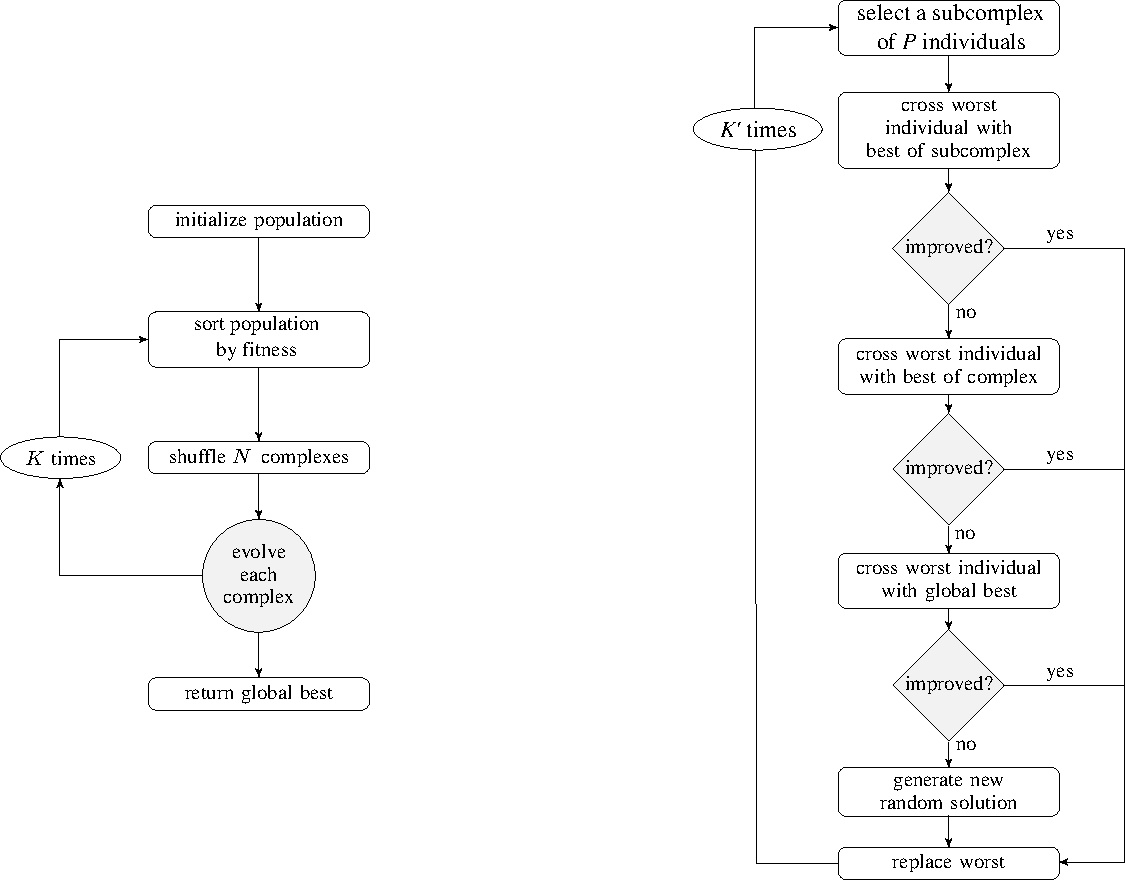
\includegraphics[scale=0.48]{sceflow}
\end{center}
\end{frame}

\section{SCE for the MKP}

\begin{frame}
	\frametitle{SCE for the MKP}
As it can be noted in its description the SCE is easily applied to any
optimization problem. \\
\vspace*{10pt}
	The only steps needed to be specified is:\\
	\qquad {\bf (a)} creation of a new random \\
	\qquad {\bf (b)} the crossing procedure of two solutions
\end{frame}

\begin{frame}
	\frametitle{The shuffled complex evolution (SCE)}
\begin{center}
		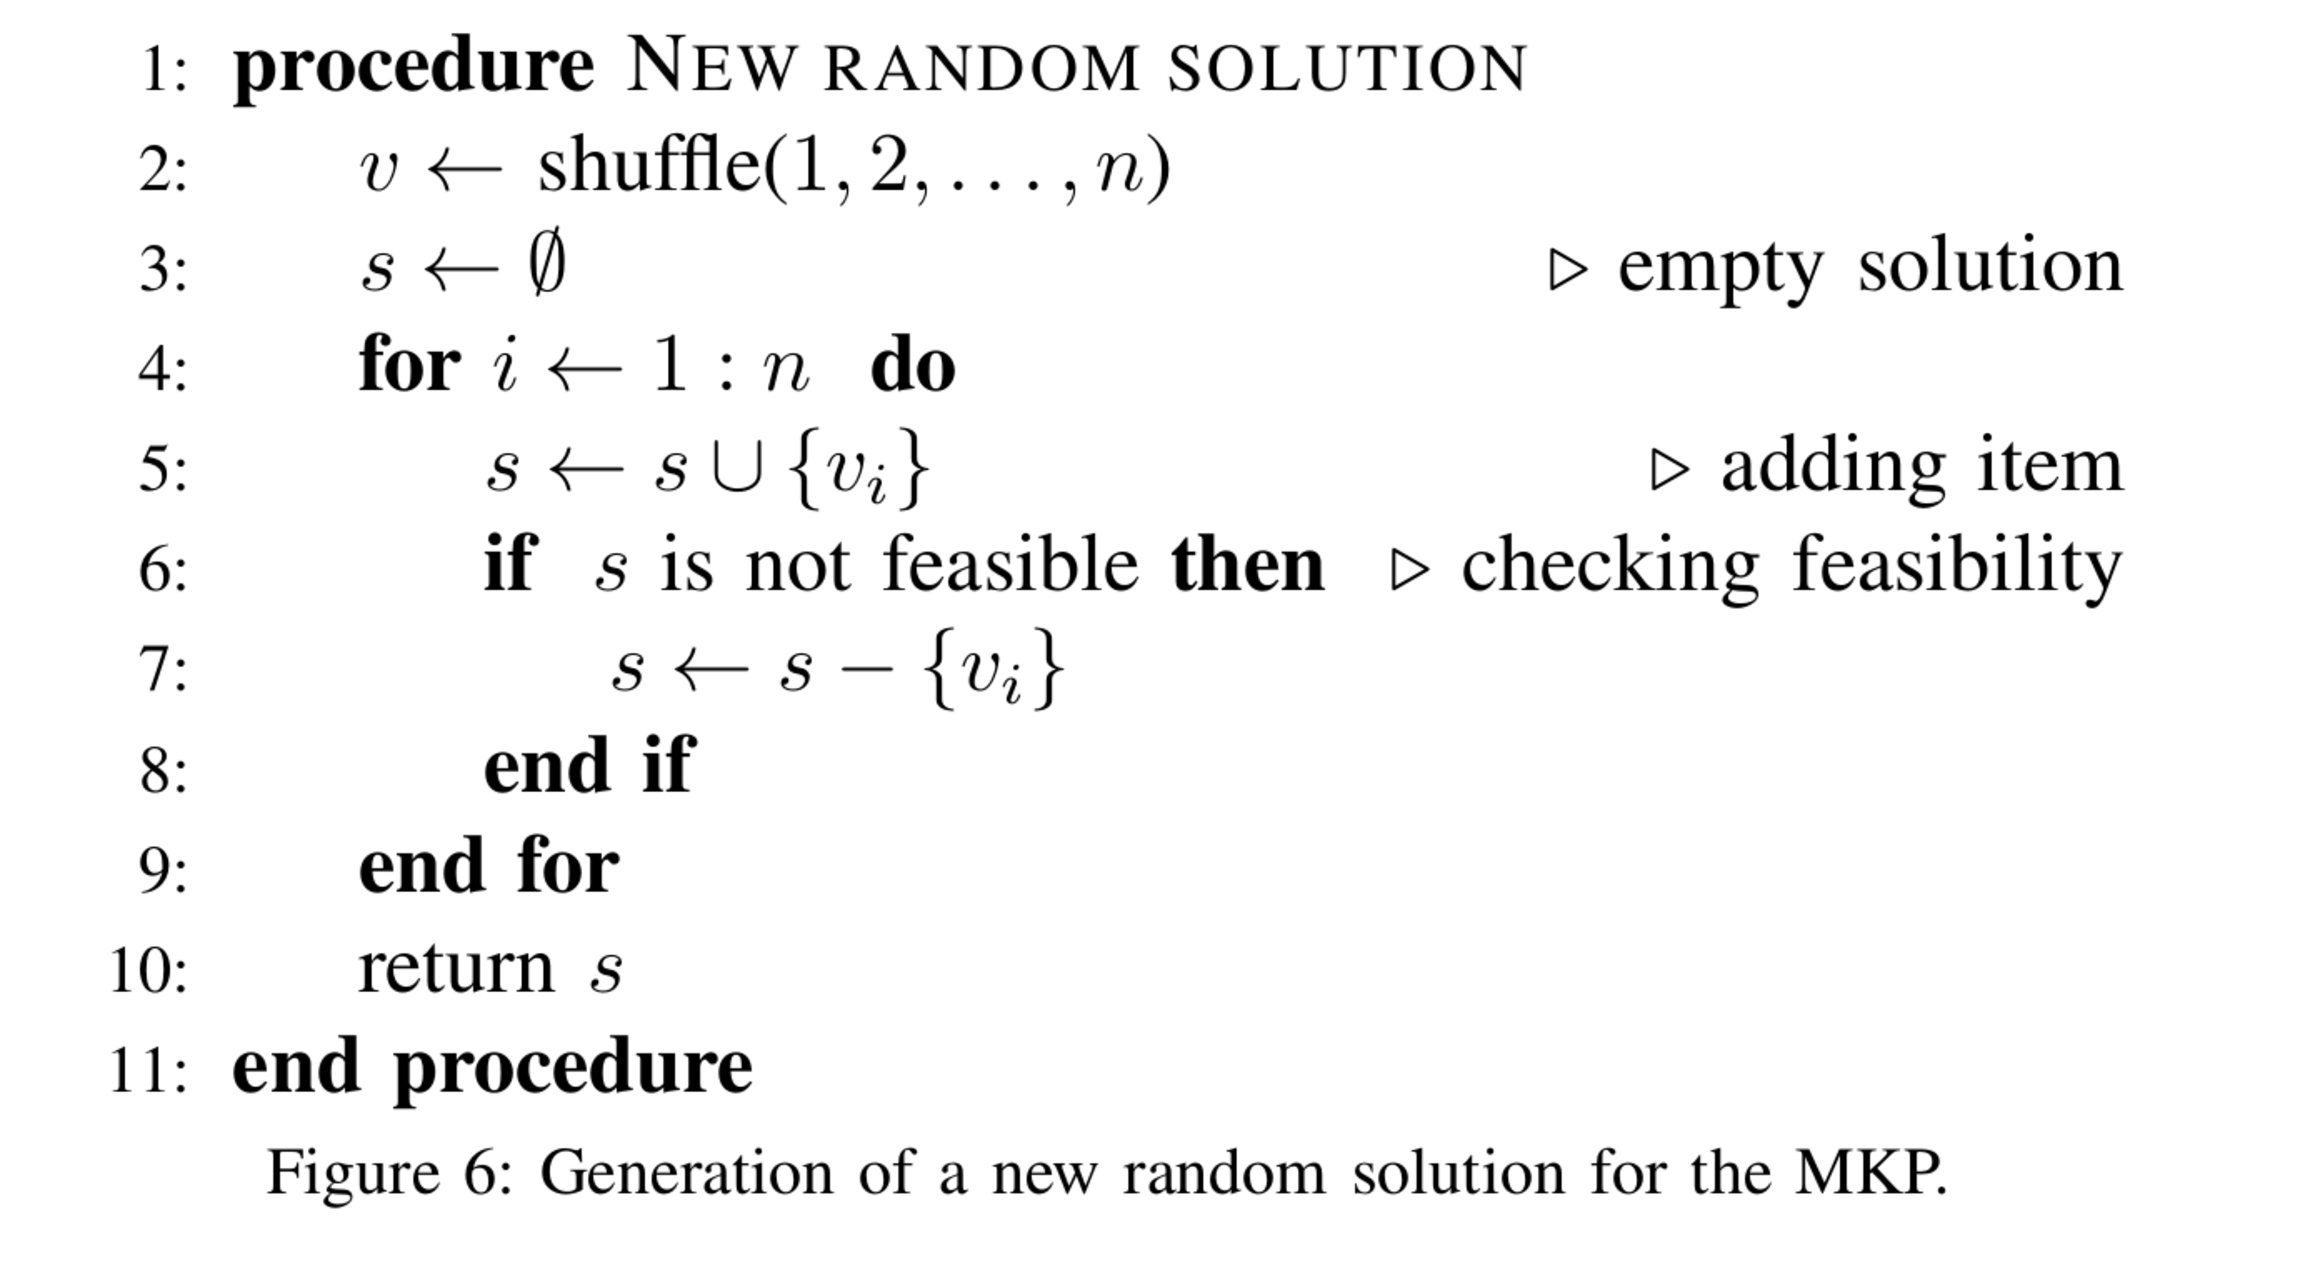
\includegraphics[scale=0.2]{rand}
\end{center}
\end{frame}

\begin{frame}
	\frametitle{The shuffled complex evolution (SCE)}
\begin{center}
		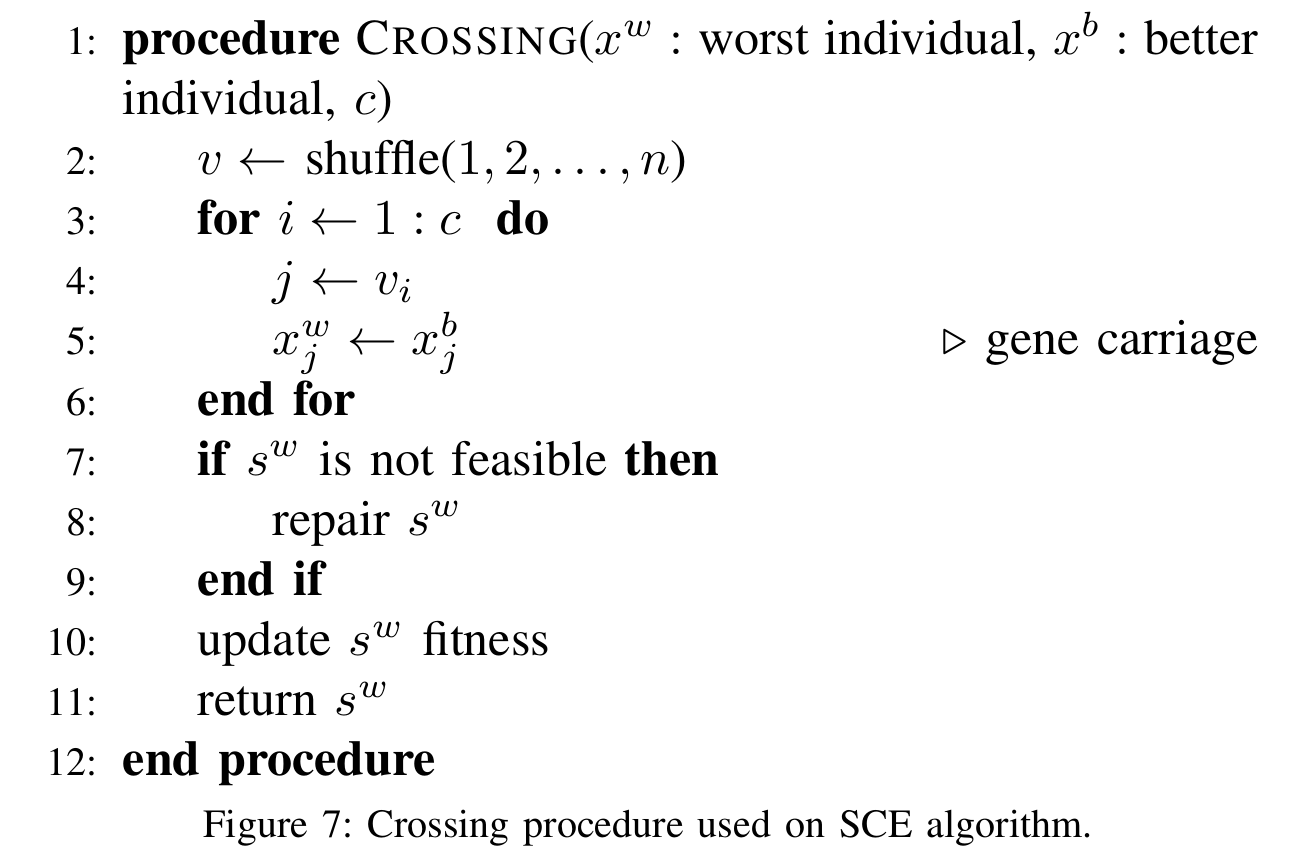
\includegraphics[scale=0.2]{cross}
\end{center}
\end{frame}

\section{Computational experiments}

\begin{frame}
	\frametitle{Computational experiments}
\begin{center}
  \begin{tabular}{c|c|l}
  \hline
  \multicolumn{1}{c}{\rule{0pt}{12pt} \bf Parameter \spc } & \multicolumn{1}{|c|}{\bf \spc Value \spc } & \multicolumn{1}{c}{\bf Description} \\[2pt]
  \hline\rule{0pt}{12pt}
  $N$  & $20$  & \spc \# of complexes \\
  $M$  & $20$  & \spc \# of individuals in each complex \\
  $P$  & $5$   & \spc \# of individuals in each subcomplex \\
  $K$  & $300$ & \spc \# of algorithm iterations \\
  $K'$ & $20$  & \spc \# of iterations for each evolving process \\
  $c$  & $n/5$ & \spc \# of genes carried (crossing) \\[2pt]
  \hline
  \end{tabular}
\end{center}
\end{frame}

\begin{frame}
	\frametitle{Computational experiments}
\begin{table}
{
\renewcommand{\arraystretch}{1.5}%
\fontsize{8.5pt}{1em}\selectfont 
\begin{center}
\begin{tabular}{|r|r|r|rr|} \hline
\textbf{n}   & \textbf{m}  & \textbf{$\alpha$} & \textbf{SCE time (s)} & \textbf{quality (\%)} \\ \hline
100 &  5 & 0.25 & 0.15 & 99.73 \\
    &    & 0.50 & 0.15 & 99.86 \\
    &    & 0.75 & 0.13 & 99.91 \\ \cline{2-5}
    & 10 & 0.25 & 0.22 & 99.53 \\
    &    & 0.50 & 0.22 & 99.76 \\
    &    & 0.75 & 0.22 & 99.96 \\ \cline{2-5}
    & 30 & 0.25 & 1.00 & 99.02 \\
    &    & 0.50 & 0.79 & 99.21 \\
    &    & 0.75 & 0.77 & 99.52 \\ \hline
    & \multicolumn{3}{r}{\textbf{average quality}}  & $\bf 99.50$  \\ \hline
\end{tabular}
\end{center}
}
 \caption{SCE performance on Chu-Beasley problems with 100 items.}
\end{table}
\end{frame}

\begin{frame}
	\frametitle{Computational experiments}
\begin{table}
{
\renewcommand{\arraystretch}{1.5}%
\fontsize{8.5pt}{1em}\selectfont 
\begin{center}
\begin{tabular}{|r|r|r|rr|} \hline
\textbf{n}   & \textbf{m}  & \textbf{$\alpha$} & \textbf{SCE time (s)} & \textbf{quality (\%)} \\ \hline
250 &  5 & 0.25 & 0.54 & 99.87 \\
    &    & 0.50 & 0.55 & 99.94 \\
    &    & 0.75 & 0.51 & 99.95 \\ \cline{2-5}
    & 10 & 0.25 & 0.67 & 99.57 \\
    &    & 0.50 & 0.62 & 99.80 \\
    &    & 0.75 & 0.64 & 99.88 \\ \cline{2-5}
    & 30 & 0.25 & 1.16 & 99.46 \\
    &    & 0.50 & 0.96 & 99.36 \\
    &    & 0.75 & 1.03 & 99.59 \\ \hline
    & \multicolumn{3}{r}{\textbf{average quality}}  & $\bf 99.60$  \\ \hline
\end{tabular}
\end{center}
}
 \caption{SCE performance on Chu-Beasley problems with 250 items.}
\end{table}
\end{frame}

\begin{frame}
	\frametitle{Computational experiments}
\begin{table}
{
\renewcommand{\arraystretch}{1.5}%
\fontsize{8.5pt}{1em}\selectfont 
\begin{center}
\begin{tabular}{|r|r|r|rr|} \hline
\textbf{n}   & \textbf{m}  & \textbf{$\alpha$} & \textbf{SCE time (s)} & \textbf{quality (\%)} \\ \hline
500 &  5 & 0.25 & 0.85 & 99.77 \\
    &    & 0.50 & 0.86 & 99.87 \\
    &    & 0.75 & 0.84 & 99.92 \\ \cline{2-5}
    & 10 & 0.25 & 0.99 & 99.49 \\
    &    & 0.50 & 0.97 & 99.78 \\
    &    & 0.75 & 0.95 & 99.83 \\ \cline{2-5}
    & 30 & 0.25 & 1.53 & 99.75 \\
    &    & 0.50 & 1.48 & 99.42 \\
    &    & 0.75 & 1.42 & 99.68 \\ \hline
    & \multicolumn{3}{r}{\textbf{average quality}}  & $\bf 99.61$  \\ \hline
\end{tabular}
\end{center}
}
 \caption{SCE performance on Chu-Beasley problems with 500 items.}
\end{table}
\end{frame}

\begin{frame}
	\frametitle{Computational experiments}
\begin{table}
{
\renewcommand{\arraystretch}{1.5}%
\fontsize{8.5pt}{1em}\selectfont 
\begin{center}
\begin{tabular}{|r|r|r|r|r|} \hline
		\textbf{\#} & \textbf{n}   & \textbf{m}  & \textbf{SCE time (s)} & \textbf{quality (\%)} \\ \hline
01 & 100 & 15 & 0.31 & 99.68 \\ \hline
02 & 100 & 25 & 0.47 & 99.51 \\ \hline
03 & 150 & 25 & 0.79 & 99.60 \\ \hline
04 & 150 & 50 & 1.61 & 99.10 \\ \hline
05 & 200 & 25 & 0.83 & 99.73 \\ \hline
06 & 200 & 50 & 1.67 & 99.30 \\ \hline
07 & 500 & 25 & 1.27 & 99.72 \\ \hline
08 & 500 & 50 & 2.06 & 99.62 \\ \hline
09 &1500 & 25 & 1.83 & 99.32 \\ \hline
10 &1500 & 50 & 5.25 & 99.76 \\ \hline
11 &2500 &100 &11.94 & 99.77 \\ \cline{1-5}
    \multicolumn{4}{|r|}{\textbf{average quality}}  & $\bf 99.46$  \\ \hline
\end{tabular}
\end{center}
}
 \caption{SCE performance on Glover-Kochenberger problems.}
 \label{tab:gk}
\end{table}
\end{frame}

\section{Conclusions and future remarks}

\begin{frame}
	\frametitle{Conclusions and future remarks}
The SCE algorithm proved to be able to achieve fast convergence ratio,
finding good quality near optimal solutions, demanding small
amount of computational time.
\vfill
The application of the core concept for MKP proved to be efficient to reduce
the size of the problems which provided fast execution time yet producing
high quality solutions.
\vfill
The heuristic could achieved $99.61\%$ on average of quality of the best known solution for
the 270 Chu-Beasley instances and $99.46\%$ on average for the Glover-Kochenberger instances.
\vfill
Future works includes the investigation of different crossing procedures 
and the use of local search in the process of evolving complexes.
\end{frame}

\begin{frame}
	\vspace*{30pt}
	\qquad \qquad {\bf Thank you!}
\end{frame}


\end{document}
